\chapter{Pressure within a Liquid}

\section{Aim}
To examine the relationship between the depth and the pressure within a liquid

\section{Background Information}
If you place a weight on your shoulders you will feel a pain which means the pressure on your body has increased. Therefore, if you were to enter into a liquid, like a lake, so that there is some liquid above you, you might think that the pressure on your body should change. Pressure in liquids is a very important topic for things like domestic water systems and dam construction. Thus, a student should find out if there is some relationship between the depth in a liquid and the pressure in the liquid at that depth, to better understand these observations. 

\section{Materials}
Tall jar can, water, bucket, 3 rubber tubes of equal length and diameter as the holes, 3 clips.

\section{Procedure}
\begin{enumerate}
\item Plug the holes of the Tall jar with rubber tubes and close the tubes with clips.
\item Fill the jar with water and then open the tubes one after the other starting with the top one.
\item Observe from each tube, how far the water travels before hitting the ground. 
\end{enumerate}

\begin{figure}[h!]
\centering
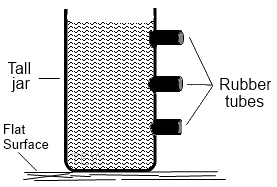
\includegraphics[width=8cm]{./img/pressure-liquid-1.png}
\caption{Pressure within a Liquid practical setup}
\label{fig:pressure-liquid-1}
\end{figure}

\section{Analysis and Interpretation}
\begin{enumerate}
\item Is there a relationship between the depth (distance from the surface of the water to the tube) of the tube and the distance traveled by the water from that tube?
\item How is the distance the liquid travels related to the speed the water leaves the tube?
\item How might the speed which the water shoots out of the rubber tube be related to the pressure in the liquid at that point?
\item How is the pressure related to the depth in the liquid?
\end{enumerate}

\section{Conclusion}
If you were discussing with another student about this experiment, how would you explain to them about the variation of pressure with depth?

\section{Questions for Discussion}
\begin{enumerate}
\item What would happen if we changed the bottle’s altitude?
\item If the diameter of the bottle was increased, but the height remained constant, would anything change in the experiment?
\item How might this experiment be related to atmospheric pressure? 
\item Would the results change if you used oil instead of water in this experiment?
\end{enumerate}

\section{Reflection and Self Assessment}
\begin{enumerate}
\item Do you feel confident that you understand the results of this experiment? If not, what can you do to improve your understanding?
\item Were you successful at completing this practical? If not, what were some of the difficulties and how might you be able to avoid them if you repeated the experiment?
\item How could you use the knowledge gained in this experiment to build a home water tank system with high pressure?
\end{enumerate}